\section*{T\'ecnicas de conteo}

\subsection*{Principio de multiplicaci\'on}

\begin{tcolorbox}[colback=blue!5!white,colframe=blue!60!black,title=Definición: Permutación]
	Una \textbf{permutaci\'on} de un conjunto es un arreglo de dichos elementos en
	alg\'un orden sin repeticiones ni omisiones.
		\label{Permutaciones_definition}
\end{tcolorbox}

Para saber el n\'umero de permutaciones que existen de un conjunto se debe
conocer su cardinalidad. Tomemos como ejemplo, el conjunto de n\'umeros enteros
$A=\{1, 2, 3\}$. Para cualquier permutaci\'on, en la primera posici\'on pueden
colocarse cualquiera de los tres elementos; en la segunda posición se pueden
colocar dos posibles elementos; mientras que al final, se puede colocar una
posibilidad.

En general, para cualquier conjunto de elementos $X$ de cardinalidad $|n|$, en
la primera posici\'on se pueden colocar $n$ elementos, para la siguiente
posici\'on $n-1$. Así sucesivamente hasta las \'ultimas posiciones, donde se
pueden colocar $3, 2$ y $1$ elementos. De esta manera, se dice que el n\'umero
de permutaciones es:

\begin{theorem}{Permutación}{permutacion}
	\begin{equation}
		P_n=n*(n-1)*(n-2)*...*3*2*1=n!
		\label{permutaciones_totales}
	\end{equation}
\end{theorem}

\subsection*{Diagrama de Árbol}
Otra forma de ver la cantidad de permutaciones de un conjunto es realizando un
diagrama de \'arbol como el de la Fig.(\ref{permutaciones_tree}).


\begin{figure}[h]
	\begin{center}		
	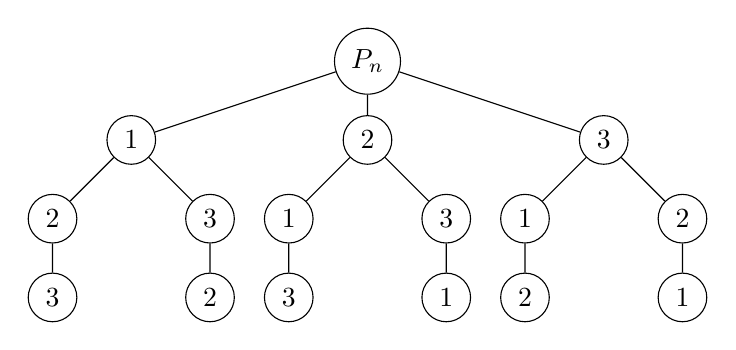
\begin{tikzpicture}[level distance=1cm, level 1/.style={sibling distance=3cm},
		level 2/.style={sibling distance=2cm}, every node/.style={circle, draw,
		align=center} ]
				\centering
				\node[circle,draw]{$P_n$}
		child{node{1} child{node{2} child{node{3}} } child{node{3} child{node{2}}} }
		child{node{2} child{node{1} child{node{3}} } child{node{3} child{node{1}}} }
		child{node{3} child{node{1} child{node{2}} } child{node{2} child{node{1}}} };
			\end{tikzpicture}
		\end{center}
		\caption{Permutaciones para 3 elementos}
		\label{permutaciones_tree}
\end{figure}

\subsection*{Permutación}

En una permutación, ocurre una \textbf{inversi\'on} cuando un elemento mayor
precede a un elemento menor. Para conocer el n\'umero de inversiones se siguen
los siguientes pasos:

\begin{itemize}
\item Tomar el primer elemento de la permutaci\'on
\item Contar los enteros menores a la derecha del elemento en cuesti\'on
\item Realizar los dos pasos anteriores para cada elemento de la permutaci\'on
\item Sumar el total de inversiones contadas para cada elemento
\end{itemize}

\textbf{Ejemplo}:

Se toma la permutación \textbf{$A=\{6,1,3,4,5,2\}$}\\

Primer elemento: $6$; menores a la derecha: $1,3,4,5,2$; n\'umero de
inversiones: \textbf{5}
Primer elemento: $1$; menores a la derecha: $\emptyset$; n\'umero de
inversiones: \textbf{0}
Primer elemento: $3$; menores a la derecha: $2$; n\'umero de inversiones:
\textbf{1}\\
Primer elemento: $4$; menores a la derecha: $2$; n\'umero de inversiones:
\textbf{1}\\
Primer elemento: $5$; menores a la derecha: $2$; n\'umero de inversiones:
\textbf{1}\\

Total de inversiones: \textbf{8}
\begin{tcolorbox}[colback=blue!5!white,colframe=blue!60!black,title=Definición: Tipos de permutaciones]
	\textbf{Permutaci\'on par:} aquella en la que el total de inversiones es un
	entero par.
	
	\tcblower

	\textbf{Permutaci\'on impar}: aquella en la que el total de inversiones es un
	entero impar.
	
\end{tcolorbox}

\subsection*{Combinación}

